\documentclass[CJKutf8,compress,hyperref]{beamer}
\setlength{\parindent}{0pt}
\setlength{\parskip}{1ex plus 0.5ex minus 0.3ex}

\usepackage{CJKutf8}
\usepackage[T1]{fontenc}
\usepackage{color}
\usepackage{beamerthemesplit} 
\usepackage{graphicx}           
\usepackage{verbatim}                              
\usepackage{listings}
\usepackage{relsize}
\usepackage{hyperref}
\usetheme{Darmstadt}                              


\setcounter{tocdepth}{3}                          
\setcounter{secnumdepth}{3}                      

\renewcommand{\today}{\number\year 年 \number\month 月 \number\day 日}

\mode<article> % only for the article version      
{                                                                          
        \usepackage{fullpage}                                          
        \usepackage{hyperref}                                         
}

\mode<presentation> { \setbeamertemplate{background canvas}
        [vertical shading][bottom=blue!8,top=blue!15]     
        \usetheme{Darmstadt}
        \usefonttheme[onlysmall]{structurebold}
}

\lstset{basicstyle=\ttfamily\tiny, keywordstyle=\color{blue!70}, commentstyle=\color{red!50!green!50!blue!50}, frame=shadowbox, rulesepcolor=\color{red!20!green!20!blue!20}, xleftmargin=2em,xrightmargin=2em, aboveskip=1em}

\begin{document}
\begin{CJK}{UTF8}{song}
        \bibliographystyle{unsrt} 
        \title{\CJKfamily{hei} Web Service简介和Axis入门指南}
        \author{\CJKfamily{hei} 吴善良}
        \institute{\CJKfamily{hei} 易保网络技术有限公司}
        \date{\CJKfamily{hei} \today}


        % \AtBeginSection[]{                              
        % \frame<handout:0>{
        % \scriptsize{\tableofcontents[current,currentsubsection]}
        % }
        % }
        %   \AtBeginSubsection[]                           
        %   {
        %   \frame<handout:0>                            
        %   {
        %       %   \frametitle{框架}
        %   \scriptsize{\tableofcontents[current,currentsubsection]} 
        % }
        % }

        \frame{\titlepage}
        \tableofcontents
        \section{\CJKfamily{hei} Web Service简介}

        \begin{frame}
                \frametitle{\CJKfamily{hei} Web Service 定义}
                \begin{itemize}

                        \item W3C(World Wide Web Consortium) 定义\cite{WebServiceDefinition}
                                \begin{itemize}
                                        \item Web服务(Web service)是一个 {\color{red}软件系统},用来支持{\color{red}网络间不同机器的互动操作}
                                        \item 服务器端会提供一个机器可读的{\color{red}接口}描述(通常基于WSDL)
                                        \item 客户端与服务端使用SOAP协议进行XML消息传递来实现互动操作
                                \end{itemize}
                \end{itemize}
        \end{frame}

        \begin{frame}
                \frametitle{\CJKfamily{hei} Web Service核心协议}
                \begin{itemize}
                        \item SOAP(Simple Object Access Protoco)\cite{SOAPTerminology}
                                \begin{itemize}
                                        \item 一种标准化通讯规范
                                        \item 基于XML的可扩展消息信封格式
                                        \item 需同时绑定一个底层通信协议(HTTP, SMTP ...)
                                        \item 规定互动的格式(RPC, 消息传递)
                                \end{itemize}
                        \item WSDL(Web services Description Language)\cite{WSDLTerminology}
                                \begin{itemize}
                                        \item 基于XML的编程接口定义语言
                                        \item 描述Web Service接口
                                        \item 可用于Web Service定位
                                \end{itemize}
                        \item UDDI(Universal Description, Discovery and Integration)\cite{UDDITerminology}
                                \begin{itemize}
                                        \item 一种目录服务
                                        \item 用于搜索,注册,发布 Web Service
                                \end{itemize}
                \end{itemize}
        \end{frame}

        \begin{frame}
                \frametitle{\CJKfamily{hei} Web Service用途}
                \begin{itemize}
                        \item 为什么要Web Service?
                                \begin{itemize}
                                        \item 可重复使用的应用程序组件
                                                \begin{itemize}
                                                        \item 服务器,客户端实现跨平台,跨语言
                                                        \item 可作为遗留系统的封装
                                                \end{itemize}      
                                        \item 更合适于B2B(Business to Business)
                                \end{itemize}
                        \item Web Service的缺点
                                \begin{itemize}
                                        \item 性能太低, 开销过大
                                        \item Web Service过于复杂
                                \end{itemize}

                \end{itemize}
        \end{frame}

        \section{\CJKfamily{hei} Axis使用入门}

        \begin{frame} 
                \frametitle{\CJKfamily{hei} Axis简介}
                \begin{itemize}
                        \item 什么是Axis?\cite{AxisIntroduction}
                                \begin{itemize}
                                        \item 本质上是一个SOAP引擎,一个构建SOAP服务器,客户端,网关等的框架
                                        \item 一个简单的独立的Web应用, 内嵌支持Servlet
                                        \item 友好地支持WSDL
                                \end{itemize}
                        \item Axis的优点
                                \begin{itemize}
                                        \item 易用性的提高
                                                \begin{itemize}
                                                        \item 提供一个简洁的传输框架实现, 支持HTTP,SMTP\ldots
                                                        \item 可自动生成WSDL文件
                                                        \item 支持从WSDL文件生成JAVA代码
                                                \end{itemize}
                                \end{itemize}
                \end{itemize}
        \end{frame}

        \begin{frame}
                \frametitle{\CJKfamily{hei} 使用Axis发布Web Service}
                \begin{enumerate}
                        \item 采用JWS(Java Web Service)文件发布
                                \begin{itemize}
                                        \item 把{\color{red}.java}文件直接拷贝到{\color{red}<your-webapp-root>/axis/}文件夹下, 并把文件后缀由{\color{red}.java}改为{\color{red}.jws}
                                        \item 简单容易, {\color{red}但是不适合程序部署和大项目开发}
                                \end{itemize}
                        \item 撰写wsdd(Web Service Deployment Descriptor)文件发布
                        \item 使用Axis提供JAVA2WSDL工具, 从JAVA代码生成WSDL文件发布服务\cite{JAVA2WSDL}
                \end{enumerate}
        \end{frame}

        \begin{frame}
                \frametitle{\CJKfamily{hei}使用WSDD发布服务端}
                \begin{enumerate}
                        \item 实现JAVA业务逻辑代码
                                \begin{itemize}
                                        \item 生成的class文件放入tomcat的classpath中
                                \end{itemize}
                        \item 为你的服务编写wsdd文件, 自定义web service部署
                        \item 使用Axis自带的工具安装wsdd文件
                                \begin{itemize}
                                        \item Axis根据wsdd文件自动为你的服务生成wsdl文件
                                \end{itemize}
                \end{enumerate}  
        \end{frame} 

        \section{\CJKfamily{hei}编写Axis的hello world例子}
        \subsection{\CJKfamily{hei}编写,发布Web Service服务端}

        \begin{frame}
                \frametitle{\CJKfamily{hei}在eclipse里创建,设置Axis服务端}
                % 整个工程目录结构如下图所示: 
                \begin{figure}[!hbp]
                        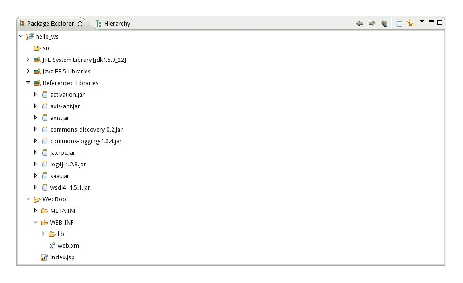
\includegraphics{hello_ws.eps}
                        %      \caption{HelloService服务端目录结构. \label{hello_ws}}
                \end{figure}
                \begin{enumerate}
                        \item 下载axis-bin-1\_4.zip, 解压
                        \item 在eclipse里创建web project, 取名hello\_ws
                        \item 把axis-1.4/lib下所有文件拷贝到hello\_ws工程WEB-INF/lib下
                        \item 把axis-1.4/webapps/WEB-INF/web.xml的内容写到hello\_ws工程WEB-INF/web.xml内
                \end{enumerate}
        \end{frame}


        \begin{frame}[containsverbatim]
        \frametitle{\CJKfamily{hei}实现一个Web Service}
        在hello\_ws项目中实现org.klose.ws.HelloWS类
        \begin{lstlisting}[language=JAVA]
        package org.klose.ws;

        public class HelloWS {
                public String sayHello(String args) {
                        return "hello " + args;
                }
        }
        \end{lstlisting}
        \begin{itemize}
                \item HelloWS本身就是一个普通的Java类
                \item 我们将在web service的客户端调用HelloWS的sayHello方法
        \end{itemize}
\end{frame}

\begin{frame}[containsverbatim]
\frametitle{\CJKfamily{hei}编写部署配置文件}
在src/org/klose/ws的目录下撰写一个简单的deploy.wsdd文件
\begin{lstlisting}[language=XML]
<?xml version="1.0" encoding="UTF-8"?>
<deployment xmlns="http://xml.apache.org/axis/wsdd/"
xmlns:java="http://xml.apache.org/axis/wsdd/providers/java">
<service name="HelloService" provider="java:RPC">
<parameter name="className" 
value="org.klose.ws.HelloWS"/>
<parameter name="allowedMethods" value="sayHello"/>
</service>
</deployment>
\end{lstlisting}
\begin{itemize}
        \item {\color{red}deployment}标签: 定义了使用到的XML Schema的命名空间
        \item {\color{red}service}标签: 定义了web service的名字, 与客户端进行互动的方式(RPC)
                \begin{itemize}
                        \item {\color{red}parameter}标签: 定义了class名字以及要公开的方法
                \end{itemize}
\end{itemize}
更多wsdd文件高级配置参见\cite{DeploymentWSDD}
  \end{frame}

  \begin{frame}[containsverbatim]
  \frametitle{\CJKfamily{hei}部署hello\_ws, 发布HelloService}
  \begin{itemize}
          \item 在eclipse中把hello\_ws项目发布到tomcat服务器上
          \item 使用{\color{red}org.apache.axis.utils.Admin}发布HelloService\cite{StaticDeployment}
                  \begin{lstlisting}[language=bash]
                  $ cd /home/klose/server/apache-tomcat-6.0.26/webapps/hello_ws/WEB-INF  
                  $ java -Djava.ext.dirs=/home/klose/Downloads/axis-1_4/lib \ 
                  >     org.apache.axis.utils.Admin server \ 
                  >     classes/org/klose/ws/deploy.wsdd 
                  \end{lstlisting}
                  \begin{itemize}
                          \item {\color{red}axis自带的jar包}必须被包含在{\color{red}classpath}内
                  \end{itemize}
          \item 用firefox打开\\
                  \small{{\color{blue}\url{http://localhost:8080/hello_ws/services/HelloService?wsdl}}}
                  如果能显示wsdl文件内容, 说明发布已经成功
  \end{itemize}
  \end{frame}

  \subsection{\CJKfamily{hei}WSDL文件说明}
  \begin{frame}[containsverbatim] 
  \frametitle{\CJKfamily{hei}HelloService.wsdl说明(一)} 
  \begin{lstlisting}[language=XML]
  <?xml version="1.0" encoding="UTF-8"?>
  <wsdl:definitions
  targetNamespace="http://localhost:8080/hello_ws/services/HelloService"
  xmlns:apachesoap="http://xml.apache.org/xml-soap"
  xmlns:impl="http://localhost:8080/hello_ws/services/HelloService"
  xmlns:intf="http://localhost:8080/hello_ws/services/HelloService"
  xmlns:soapenc="http://schemas.xmlsoap.org/soap/encoding/"
  xmlns:wsdl="http://schemas.xmlsoap.org/wsdl/"
  xmlns:wsdlsoap="http://schemas.xmlsoap.org/wsdl/soap/"
  xmlns:xsd="http://www.w3.org/2001/XMLSchema">
  ........
  </wsdl:definitions>
  \end{lstlisting}
  定义了wsdl文件使用到的各个命名空间
  \end{frame}

  \begin{frame}[containsverbatim] 
  \frametitle{\CJKfamily{hei}HelloService.wsdl说明(二)} 
  \begin{lstlisting}[language=XML]
  <wsdl:message name="sayHelloRequest">
  <wsdl:part name="args" type="xsd:string" />
  </wsdl:message>
  <wsdl:message name="sayHelloResponse">
  <wsdl:part name="sayHelloReturn" type="xsd:string" />
  </wsdl:message>

  <wsdl:portType name="HelloWS">
  <wsdl:operation name="sayHello" parameterOrder="args">
  <wsdl:input message="impl:sayHelloRequest"
  name="sayHelloRequest" />
  <wsdl:output message="impl:sayHelloResponse"
  name="sayHelloResponse" />
  </wsdl:operation>
  </wsdl:portType>
  \end{lstlisting}
  \begin{itemize}
          \item  {\color{red}wsdl:message} 通过消息方式传递的参数和返回值  
                  \begin{itemize}
                          \item {\color{red}wsdl:part} 每个参数在这条消息中对应的变量名字和变量类型
                  \end{itemize}
          \item {\color{red}wsdl:portType} 一个web service里可以被调用方法的集合
                  \begin{itemize}
                          \item {\color{red}wsdl:operation} 一个可以公开被调用的方法, 调用时需要的传递的消息,调用结束返回的消息
                  \end{itemize}
  \end{itemize}
  \end{frame}

  \begin{frame}[containsverbatim] 
  \frametitle{\CJKfamily{hei}HelloService.wsdl说明(三)} 
  \begin{lstlisting}[language=XML]
  <wsdl:binding name="HelloServiceSoapBinding" type="impl:HelloWS">
  <wsdlsoap:binding style="rpc"
  transport="http://schemas.xmlsoap.org/soap/http" />                       
  <wsdl:operation name="sayHello">
  <wsdlsoap:operation soapAction="" />                      
  <wsdl:input name="sayHelloRequest">
  <wsdlsoap:body
  encodingStyle="http://schemas.xmlsoap.org/soap/encoding/"
  namespace="http://ws.klose.org" use="encoded" />
  </wsdl:input>   
  <wsdl:output name="sayHelloResponse">
  <wsdlsoap:body
  encodingStyle="http://schemas.xmlsoap.org/soap/encoding/"
  namespace="http://localhost:8080/hello_ws/services/HelloService"
  use="encoded" />
  </wsdl:output>
  </wsdl:operation>
  </wsdl:binding>
  \end{lstlisting}
  \begin{itemize}
          \item  {\color{red}wsdl:binding} 描述消息构成,消息传递有关协议的信息
                  \begin{itemize}
                          \item {\color{red}wsdlsoap:binding} 消息格式符合soap协议(get, post\ldots)
                                  \begin{itemize}
                                          \item {\color{red}style="rpc"} soap消息式样为rpc(document\ldots)
                                          \item {\color{red} transport="http://schemas.xmlsoap.org/soap/http} \\ 消息传递协议为http(smtp\ldots)
                                  \end{itemize}
                  \end{itemize}
  \end{itemize}
  \end{frame}

  \begin{frame}[containsverbatim] 
  \frametitle{\CJKfamily{hei}HelloService.wsdl说明(四)} 
  \begin{lstlisting}[language=XML]
  <wsdl:service name="HelloWSService">
  <wsdl:port binding="impl:HelloServiceSoapBinding"
  name="HelloService">
  <wsdlsoap:address
  location="http://localhost:8080/hello_ws/services/HelloService" />
  </wsdl:port>
  </wsdl:service>
  \end{lstlisting}
  \begin{itemize}
          \item {\color{red}wsdl:service} web service的名字, 一个web service由多个port组成
                  \begin{itemize}
                          \item {\color{red}wsdl:port} wsdl:port等于wsdl:portType + wsdl:binding
                          \item 同一个wsdl:portType可以使用不同的wsdl:binding方式
                                  \begin{itemize}
                                          \item {\color{red}wsdlsoap: address} 对应于port的url调用地址
                                  \end{itemize}
                  \end{itemize}
  \end{itemize}
  \end{frame}

  \subsection{\CJKfamily{hei}生成Web Service客户端}
  \begin{frame}[containsverbatim]
  \frametitle{\CJKfamily{hei}基于Axis编写Web Service客户端代码} 
  \begin{lstlisting}[language=JAVA]
  import javax.xml.namespace.QName;
  import org.apache.axis.client.Call;
  import org.apache.axis.client.Service;
  public class Client {
          public static void main(String[] args) {
                  try {
                          String endpoint = "http://localhost:8080/hello_ws/services/HelloService";
                          Service service = new Service();
                          Call call = (Call) service.createCall();
                          call.setTargetEndpointAddress(new java.net.URL(endpoint));
                          call.setOperationName(new QName("http://ws.klose.org", "sayHello"));
                          String ret = (String) call.invoke(new Object[] { "world" });
                          System.out.println(ret);
                  } catch (Exception e) {
                          System.err.println(e.toString());
                  }
          }
  }
  \end{lstlisting}
  \begin{itemize}
          \item {\color{red}\emph{call.setTargetEndpointAddress}} \small{设定要调用的web service的url}
          \item {\color{red}\emph{call.setOperationName}} \small{设定要调用的方法命名空间以及名字}
          \item {\color{red}\emph{call.invoke}} \small{传递参数, 调用web service}
  \end{itemize}
  \end{frame}

  \begin{frame}[containsverbatim] 
  \frametitle{\CJKfamily{hei}使用Axis工具生成Web Service客户端}
  \begin{enumerate}
          \item 下载生成的wsdl文件
                  \begin{lstlisting}[language=bash]
                  $ mkdir -p ~/tmp/client/ 
                  $ cd ~/tmp/client/ 
                  $ wget "http://localhost:8080/hello_ws/services/HelloService?wsdl" \ 
                  >    -O HelloService.wsdl 
                  \end{lstlisting}
          \item 使用{\color{red}WSDL2Java}生成HelloService客户端代码\cite{WSDL2JAVA}
                  \begin{lstlisting}[language=bash]
                  $ java -Djava.ext.dirs=/home/klose/Downloads/axis-1_4/lib \ 
                  >    org.apache.axis.wsdl.WSDL2Java \ 
                  >     -p org.klose.ws HelloService.wsdl 
                  \end{lstlisting}
                  \begin{itemize}
                          \item {\color{red}-p}: 把生成的代码放在{\color{red}./org/klose/ws}下面, 不使用wsdl文件中的namespace来生成目录结构
                  \end{itemize}
  \end{enumerate}
  \end{frame}

  \begin{frame}[containsverbatim] 
  \frametitle{\CJKfamily{hei}测试生成的HelloService客户端代码} 
  \begin{enumerate}
          \item 在eclispe中创建java project, 取名hello\_ws\_client
          \item 导入刚才生成的代码
          \item 引用下载的axis/lib中的jar包
          \item 编写org.klose.ws.client.HelloServiceClient类 
  \end{enumerate}
  \end{frame}

  \begin{frame} 
          \frametitle{\CJKfamily{hei}生成代码的UML类图}
          \begin{figure}[!hbp]
                  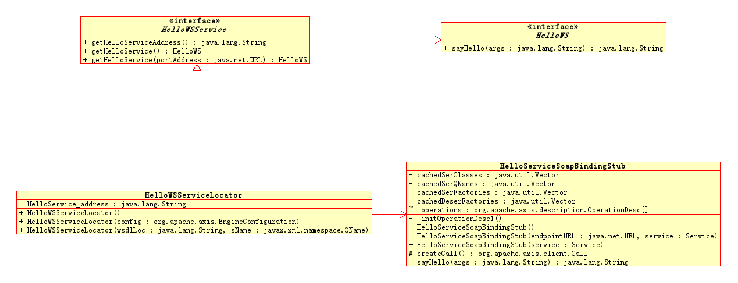
\includegraphics{class_diagram.eps}
                  %      \caption{HelloService客户端UML类图. \label{class_diagram}}
          \end{figure}
          \begin{itemize} 
                  \item {\color{red}HelloServiceSoapBindingStub} 辅助类,实现binding细节
                  \item {\color{red}HelloWSService} web service接口, 用来获取port
                  \item {\color{red}HelloWSServiceLocator} 实现web service接口
                  \item {\color{red}HelloWS} port, 用来调用operation
          \end{itemize}
  \end{frame}

  \begin{frame}[containsverbatim]
  \frametitle{\CJKfamily{hei}HelloServiceClient代码 }
  \begin{lstlisting}[language=JAVA]
  package org.klose.ws.client;
  import java.rmi.RemoteException;
  import javax.xml.rpc.ServiceException;
  import org.klose.ws.HelloWS;
  import org.klose.ws.HelloWSService;
  import org.klose.ws.HelloWSServiceLocator;
  public class HelloServiceClient {
          public static void main(String[] args) {
                  HelloWSService service = new HelloWSServiceLocator();
                  try {
                          HelloWS port = service.getHelloService();
                          System.out.println(port.sayHello("world"));
                  } catch (ServiceException e) {
                          e.printStackTrace();
                  } catch (RemoteException e) {
                          e.printStackTrace();
                  }
          }
  }
  \end{lstlisting}
  运行这个Java类进行测试. 
  \end{frame} 

  \section{\CJKfamily{hei}总结} 
  \begin{frame}
          \frametitle{\CJKfamily{hei}Web Service总结}
          \begin{itemize}
                  \item 支持SOA(面向服务)的架构
                          \begin{itemize}
                                  \item 可自发发布, 被使用, 被发现
                          \end{itemize}
                  \item 开发, 部署, 使用Web Service
                          \begin{itemize}
                                  \item 能与现有的编程语言(JAVA, .NET\ldots)整合 
                                  \item WSDL作为Web服务的“接口定义语言”
                                          \begin{itemize} 
                                                  \item WSDL$\rightarrow$编程语言: 发布新的Web服务, 自动产生服务端代码
                                                  \item 编程语言$\rightarrow$WSDL: 封装原有的组件, 以Web服务发布
                                          \end{itemize}
                          \end{itemize}
                  \item SOAP 
                          \begin{itemize}
                                  \item 客户端和服务端互动传递消息的格式
                                  \item 基于XML 
                                  \item 独立于消息传递协议
                                  \item 可以绑定于不同互动式样
                                  \item 提供扩展性, 错误处理机制, 以及用户自定义的类型支持
                          \end{itemize} 
          \end{itemize}
  \end{frame} 

  \section{\CJKfamily{hei}致谢}
  \begin{frame}
          \begin{Huge}
                  \begin{center}
                          谢谢大家的聆听!
                  \end{center}
          \end{Huge}
  \end{frame}
  \bibliography{axis.bib} 
\end{CJK}
\end{document}
